% !TEX root = main.tex

%%%%%%%%%%%%%%%%%%%%%%%%%%%%%%%%%%%%%%%%%%%%%%%%%%%%%%%%%%%%%%%%%%%%%%%%%%%%%%%%
\chapter{Proposed contributions}
% Metho!


% Clear that the community has an interest
From the overwhelming positive reviews and great comments we received for our previous work, it seems clear to me that the community is interested in outdoors PS. Reviewers found the work ``refreshing'', praising its ``concrete actionable predictions that can be of interest for practitioners'' and the pertinence of this line of work. Based on this feedback from the community, I look forward to build upon the existing contributions.

% Based on the work already done
Previous contributions mainly focused on the analysis of the complex illumination conditions of outdoor scenes. This analysis brought us a good deal of knowledge that will enable the enhancement of existing reconstruction algorithms.

But first, something is missing among the community to continue experiments with outdoor PS: a database of diverse objects publicly available. Just as the sky database we built, I propose to capture and share unsaturated HDR images of objects under various natural illumination conditions.

Then, using this database and the previous work we did, I will be able to modify existing PS algorithms to work for outdoor conditions. This work will be split in steps: first, I'll tackle the case when the illumination is known and gradually move toward the case where only some object images are required. This includes merging ideas from other 3D reconstruction techniques to simplify the problem or correct some issues that PS is not able to fix in the general case.

After having improved existing PS reconstruction algorithms using knowledge from the day lit sky, I'll focus on the other things a practitioner could consider and do to make PS work in problematic cases.


\section{Database of objects}

As explained previously (\ref{sec:hdrdb}), after realizing that the research community was missing one, we've built a publicly available database of unsaturated HDR sky captures. This led to the realization that something else is missing: the same database, but for objects instead of skies. This database would allow researchers to analyze the shading of surfaces in conjunction with their illumination conditions. The goal is to obtain and share pictures of objects synchronized with the sky captures. These images will effectively give a direct link between the aspect of a sky and the appearance of objects lit by it. More importantly for this current project, it will also give the inverse: given a picture of an object, what sky lit it.

% Cite AMOS http://amos.cse.wustl.edu/
Similar databases already exist in the community (e.g., AMOS~\cite{jacobs-cvpr-2007}, Yahoo!'s databases~\cite{thomee-arxiv-15}), leading one to believe that this kind of data is wanted and appreciated by the researchers. Data available is usually very rich, yielding a lot of different content and objects with various reflectances. The issue of this data, for this thesis, is the lighting conditions. A full HDR capture of the sky synchronized with the images is not available. Furthermore, it is often difficult to estimate what the illumination looked like. Images may, or may not, have GPS coordinates, sometimes with the wrong information. Date and time in the EXIF data of the images are often wrong or skewed. Camera orientation (such as azimuth) is mostly never provided with these databases. As such, it is then hard to guess the position of the sun in the sky. These databases are really interesting to test an uncalibrated reconstruction technique, but something is missing for its development.

% small & big
The idea of the database would be to gather images of various objects. At first, simple matte surfaces will be the focus, since they are simpler to work with. Objects with more complex reflectances will come later on. Two key characteristics are important for this analysis: small and big objects. Small objects are mandatory, because it is possible to easily obtain a ground truth mesh from them using a handheld 3D scanner. Having a ground truth will greatly help the development of reconstruction algorithm and the measurement of its performance. Big objects are also important, because they are the main interest of using outdoor PS. To scan building-scale objects, handheld 3D scanners require quite a long time to operate, making them impracticable in this case. On the long term, reconstructing such big objects, like statues and buildings, is the goal set to achieve in this thesis. Having the data ready to perform the rest of the project is a logical step in the right direction. This database is the answer to this need.

% Build on existing infrastructure
A lot of effort is required to build and share a new dataset. This is why I plan on reusing the infrastructure we already have for the sky database. The capture system is already available, as well as the publishing interface. Two things are left to do. First, taking the captures and move them to the existing infrastructure. Then, some minor modifications of the current infrastructure will be required, as it is currently focused on sky captures only. The goal is to be as efficient as possible and put the minimum effort into the system \emph{per se} to focus on the objects to be captured their reconstruction.

% Technical side
On the technical side, a Canon 5D mark III camera will be used in addition to the system already in place for the sky capture described in \ref{sec:hdrdb}. This additional camera will perform 5 burst captures of the object, in order to gather all the information needed to build an unsaturated HDR photo. A small chrome sphere is inserted in this camera's field of view to allow calibration with the sky camera. Hence, the precise rotation will be known between both cameras. A system based on ROS developed by interns\footnote{Available publicly at \url{https://github.com/lvsn/CameraNetwork}} orchestrates the camera network and synchronizes the captures among cameras.


\section{Calibrated outdoor reconstruction}
\label{sec:calib}

% Up to now, only analysis. Make something with it.
Until now, the work done in the previous contributions revolves around the analysis of natural skies. The next step is to use this new knowledge to build a reconstruction algorithm. At first, many simplifications will be done to the problem to be able to modify an existing algorithm and make it work outside. Here are described what I want to achieve first, followed by the insights that will make it work.

% Calibrated case.
In the beginning, the whole sky is assumed to be known to the algorithm as well as its calibration with respect to the object pictures. This means that the MLV matrix $\bar{L}$ can be known \emph{a priori}, given the right normals. Object surfaces are assumed to be Lambertian, but are not required to be constant. While complex reflectances could be found relatively easily from the sky capture -- the environment map --, assuming Lambertian reflectance is be necessary for the upcoming uncalibrated version of the algorithm, discussed later.

The images must all be aligned. Image alignment or registration is another field of study which is solved for the case useful for PS. This is discussed in~\cite{ackermann-cvpr-12}, as previously explained. I will suppose the images were already aligned using such technique in the proposed algorithm.

% Explain the DLT
In the basis algorithm I plan to build upon, there are two important enhancements from the original PS algorithm as defined originally. First, it is possible to remove the albedo $\rho$ from the equation to cancel the effect of the surface reflectance, making the algorithm robust to albedo variability. Secondly, instead of solving for the normals, it is possible to solve for the surface height directly. 

To remove the albedo $\rho$ from the original PS equation, the trick is to divide an image by another one. Mathematically, this pixelwise division of, let's say, image 1 by image 2, is represented as

\begin{equation}
\frac{b_{t,1}}{b_{t,2}} = \frac{\rho_t \mathbf{l}_1 \mathbf{n}_t}{\rho_t \mathbf{l}_2 \mathbf{n}_t} \quad,
\end{equation}
for pixel $t$. The albedo $\rho_t$ cancels out, giving the relation
\begin{equation}
\label{eq:ratio_images}
\left( b_{t,1} \mathbf{l}_2 - b_{t,2} \mathbf{l}_1 \right) \mathbf{n}_t = 0  \quad.
\end{equation}

This relation was used before~\cite{yu-iccp-13,wu-pami-06}. These algorithm usually consist of taking a denominator image minimally affected by shadows and highlights and dividing all the other images of the sequence by this one. While this removes the constant albedo assumption, it leaves a smaller (by one) sequence of images to perform PS. Another possibility is to perform the division on all the possible permutations of images, giving a better robustness to the algorithm. The problem with this approach is that it makes the sequence grow quadratically (see appendix \ref{anx:permutations}), which quickly becomes problematic to solve in a reasonable time on computers having a finite amount of memory. Stochastically taking a predetermined amount can do the trick, but a more sound selection is discussed later on.
 
Solving directly for the surface height instead of the normals can be done by analyzing the relation between both. Given pixel $t$ and its depth $z_t$, the normal of the surface patch seen by it $\mathbf{n}_t$ can be expressed as
\begin{equation}
r_t = 
\begin{bmatrix}
\nabla z_{t,x} \\
\nabla z_{t,y} \\
-1
\end{bmatrix}
\end{equation}
\begin{equation}
\mathbf{n}_t =
\frac{r_t}{\norm{r_t}} \quad.
\end{equation}
This supposes that the surface is pointing toward $-1$, hence the camera is at $[0, 0, -1]$.

When merged with the albedo removal technique (equation \eqref{eq:ratio_images}) and letting down the normalization, we obtain
\begin{equation}
\label{eq:pre-dlt}
\left( b_{t,1} \mathbf{l}_2 - b_{t,2} \mathbf{l}_1 \right)
\begin{bmatrix}
\nabla z_{t,x} \\
\nabla z_{t,y} \\
-1
\end{bmatrix}
= 0  \quad.
\end{equation}

This version of PS is the base upon which the proposed enhancements are planned. In order to make it easier to handle, a Direct Linear Tranform (DLT) method is applied to rewrite equation~\eqref{eq:pre-dlt} into an set of homogeneous linear equations.

To do so, we must consider the left part of the equation, $\left( b_{t,1} \mathbf{l}_2 - b_{t,2} \mathbf{l}_1 \right)$, as being a vector of three scalars, let's say $\left[ i_t, j_t, k_t \right]$. When considering the division of an image $a$ by $a'$ as a whole instead of looking at each pixels separately, we get the vectors $\left[ \mathbf{i}_{aa'}, \mathbf{j}_{aa'}, \mathbf{k}_{aa'} \right]$. Equation \eqref{eq:pre-dlt} can now be rewritten as
\begin{equation}
\left[ \mathrm{diag}(\mathbf{i}_{aa'}) \; \mathrm{diag}(\mathbf{j}_{aa'}) \; \mathrm{diag}(\mathbf{k}_{aa'})\right]
\begin{bmatrix}
\nabla \mathbf{z}_{x} \\
\nabla \mathbf{z}_{y} \\
-1
\end{bmatrix}
= 0 \quad,
\end{equation}
which can be rewritten as
\begin{equation}
\left[ \mathrm{diag}(\mathbf{i}_{aa'}) \; \mathrm{diag}(\mathbf{j}_{aa'}) \right]
\begin{bmatrix}
\nabla \mathbf{z}_{x} \\
\nabla \mathbf{z}_{y} \\
\end{bmatrix}
= \mathbf{k}_{aa'} \quad.
\end{equation}

In order to convert this independent systems of linear equations into an homogeneous form, it is possible to arrange this matrix into a block diagonal matrix by taking each row and making $2x2$ blocks from them.
This gives this new formulation:
\begin{equation}
\sum_{a,a'}
\begin{bmatrix}
D_{ii} & D_{ij} \\
D_{ij} & D_{jj} \\
\end{bmatrix}_{a,a'}
z =
\sum_{a,a'}
\begin{bmatrix}
D_i \mathbf{k} \\
D_j \mathbf{k} \\
\end{bmatrix}_{a,a'}
\quad,
\end{equation}
where $D_i = \mathrm{diag}(\mathbf{i}_{aa'})$ and $ D_{ij} = \mathrm{diag}\left(\mathbf{i}_{aa'} \circ \mathbf{j}_{aa'}\right)$ ($\circ$ being the elementwise, or Hadamard, product). This gives the DLT formulation of the PS problem with the two explained enhancements.

% Normalization
%This formulation of PS has a problem. Since the first line is multiplied by $D_i$ and the second by $D_j$, the conditioning of this system is then also squared, which is not desirable. 

% What's coming up next
Four avenues will be discussed on how I plan to make this PS algorithm work for outdoors. First, using the observations we made in our analysis brought us some ideas on how to improve the reconstruction performance. Two of such ideas are discussed. Then, interesting elements found in other algorithms and their inclusion in the proposed algorithm will be explained.

\subsection{Regularization}

% One thing we noticed during our analysis is that not all pixels nor axis are equal.
% Figure, axis uncertainty
During our analysis, we noticed that not all pixel have the same uncertainty. Certain portions of the sphere were more prone to exhibit erratic reconstructions than others. Moreover, we found that a single pixel would often have a different uncertainty depending on its direction. This means that a normal recovered from a pixel could have a high accuracy on its azimuth and be very inaccurate on its elevation. This is a direct effect of natural lighting conditions variations over the image sequence.

We could leverage this information by performing regularization. Regularization is a type of prior we can put into the problem to favor some kind of solution over others. The kind of solution to be favored is chosen arbitrarily. In the case of object surfaces, a prior often made is the assumption of smoothness. This means that the optimization will be biased toward smooth solutions, i.e.\ not having abrupt curves. This is the prior that will be used for the rest of the section.

Two types of regularization exist: isotropic and anisotropic. Isotropic regularization means enforcing the same penalty for abrupt changes regardless of the direction, whether on the $x$ or the $y$ axis. Anisotropic regularization is the contrary: penalty won't be the same depending on which axis the roughness lies. The same irregularity may give a completely different penalty depending on which axis it lies on.

This idea was exploited in~\cite{hernandez-pami-11}, where they used first and second order anisotropic shape regularization on PS. They worked on the case where the sequence of images is limited to two images, or analogously three image with one of which is partially in shadow. This case led them to define the characteristic curve as the constraint induced by two lights, meaning a curve that has one degree of freedom. All the pixels lying on this curve are constrained in one direction (along the characteristic curve), but have no information on the other direction. An example of such curves is show in fig.~\ref{fig:reg-her3}.

\begin{figure}
\centering
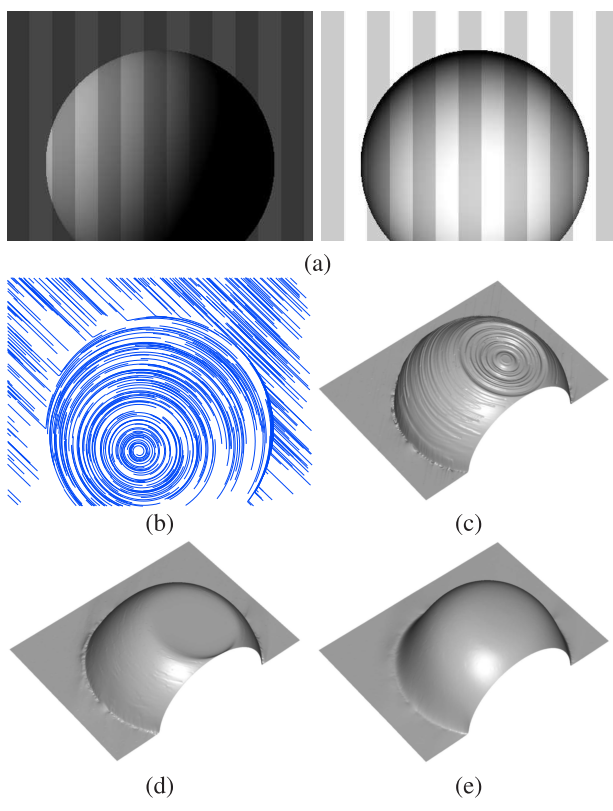
\includegraphics[height=8cm]{Regularization/hernandez_fig3.png}
\caption{Two-source photometric stereo with varying albedo. \textbf{(a)} shows the two input images. \textbf{(b)} shows the characteristic curves obtained by plotting the seeds following the 2D flow. \textbf{(c)} shows one possible reconstruction. Note how each curve is reconstructed independently because of a lack of constrain across neighboring curves. \textbf{(d)} and \textbf{(e)} shows reconstruction using anisotropic regularization, with $\alpha = 0.1, \beta = 0$ and $\alpha = 0, \beta = 0.5$, respectively. Figure from~\cite{hernandez-pami-11}}
\label{fig:reg-her3}
\end{figure}

In order to deal with this undesired extra degree of freedom, they choose to perform shape regularization. Without regularization, the results may be quite far from the ground truth~\ref{fig:reg-her2}. 

\begin{figure}
\centering
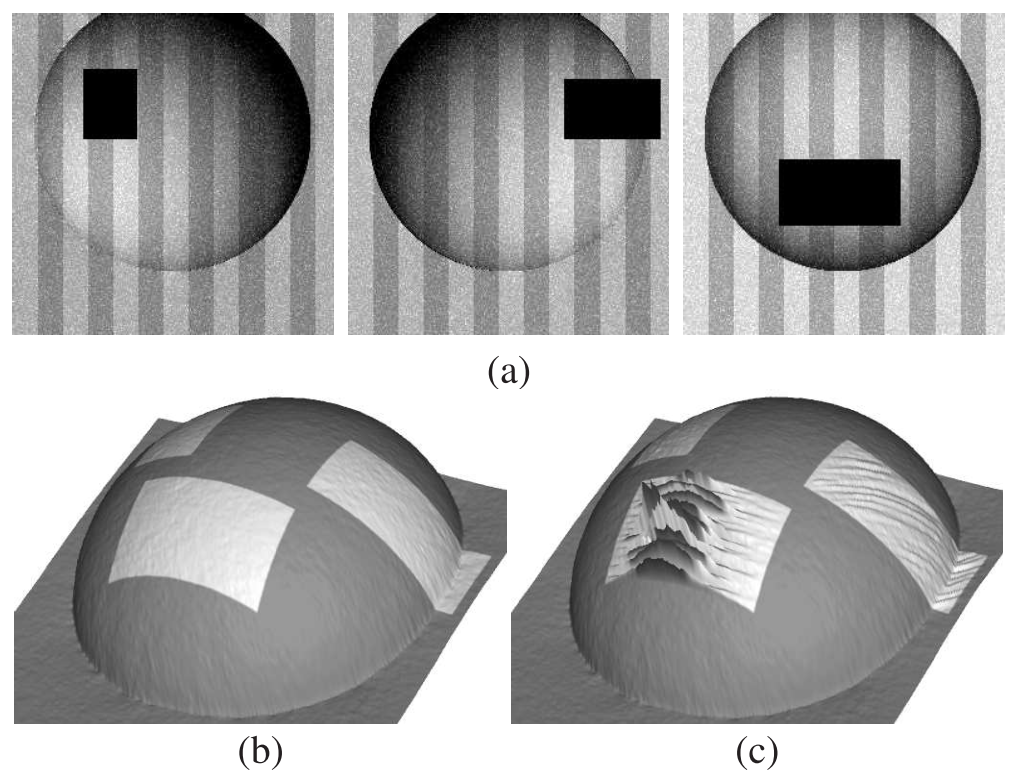
\includegraphics[height=8cm]{Regularization/hernandez_fig2_abc.png}
\caption{Experiment on shadowed input. \textbf{(a)} input images. \textbf{(b)} Ground truth, reconstruction performed without shadows. \textbf{(c)} Reconstruction performed with the shadows. The lighter zones represents the shadows. Figure from~\cite{hernandez-pami-11}}
\label{fig:reg-her2}
\end{figure}

In the case of two-source PS, the regularization must be performed along directions that are perpendicular to the characteristic curves, let's call them $\mathbf{u}$. Hence, the regularization they use is of the form
\begin{equation}
\alpha \lvert \mathbf{u}^T \nabla z \rvert ^2
\end{equation}
for the first order, and 
\begin{equation}
\beta \lvert \mathbf{u}^T H(z)\nabla z \rvert ^2
\end{equation}
for the second order, where $z$ is the height, $\alpha$ and $\beta$ are the regularization weights and $H(z)$ is the Hessian matrix of $z$ (its second-order derivatives). While the first order penalizes non-smooth the slopes, the second order penalizes non-smooth curvatures.

While the idea is similar, the problem of regularizing in function of the normal uncertainty is a bit different. When the pixel normal uncertainty is inferred directly from the lighting, it won't be in a purely single direction as in the case of \cite{hernandez-pami-11}. The uncertainty may be any combination of two orthogonal vectors, and may even end up having an isotropic behavior (i.e., the uncertainty is equal in both directions). As such, the $\mathbf{u}$ vector must be changed to $\mathbf{u}(x,y)$, with $x$ and $y$ being the coordinates in pixel-space.

We can simplify $\mathbf{u}(x,y)$ to a set of two orthogonal vectors along both axes. Since the uncertainty is computed directly on the $x$ and $y$ axes, we can rewrite the regularization as a linear combination of these two vectors:
\begin{equation}
\alpha \lvert \mathbf{u}_x \nabla z + \mathbf{u}_y \nabla z\rvert ^2 +
\beta \lvert \mathbf{u}_x H(z)\nabla z + \mathbf{u}_y H(z)\nabla z\rvert ^2
\quad,
\end{equation}
where $\mathbf{u}_x$ and $\mathbf{u}_y$ are the perpendicular components of the uncertainty.

This new formulation is still untested. As such, my plan is to incorporate it into the reconstruction algorithm and to monitor its performance improvements. Something that is not taken into account as of now are the edges. Two pixels having two completely different intensities over the image sequence indicate that their normals should be quite far apart and thus should not be strongly regularized for smoothness. Such a regularization is used in~\cite{jung-cvpr-15} and discussed later.


\subsection{Selection and scaling}
% Discrepancy between simulation and real world captures. Investigate it. We witness: selecting some images of the sequence may improve or degrade dramatically reconstruction performance.
While working on the previous contributions, we witnessed a strange behavior in the reconstruction performance. Two symptoms were noticed, which -- we believe -- come from the same root, and will be solved by a single solution.

First, simulations on cloudy and semi-cloudy lighting conditions reflected correctly the real captured data. But when the sun was directly visible by a surface patch, a drift in the intensity values was observed compared to the theory. Pixels seeing direct bright sunlight were typically dimmer than what the Lambertian equation predicted, as can be seen in fig.~\ref{fig:sel-scaling_error}. This situation is corroborated by the real data. In itself, this minor setback won't hinder the forecast work. It seems to suppose that our real objects does not exhibit perfectly Lambertian reflectances, which is not quite surprising, and is something that the physically-based renderer LuxRender also picks up. The important thing to keep in mind from this is that images lit by direct sunshine will impact negatively the performance of the PS algorithm.

\begin{figure}
\centering
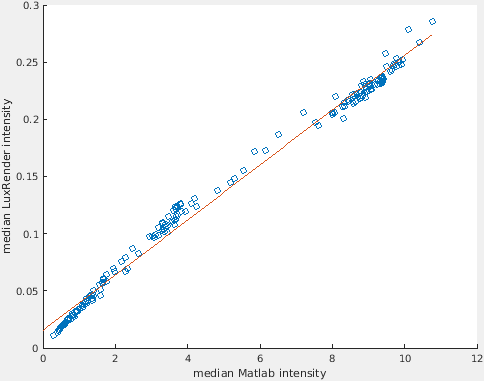
\includegraphics[height=8cm]{selection_scaling/intensity_sphere_lux_lin.png}
\caption{Median intensity of rendered images. The physically-based renderer LuxRender ($y$-axis) is compared against the Lambertian equation ($x$-axis). The same material and light directions are used in both rendering methods. A linear best fit is shown in red. As it can be seen, the curve is not perfectly linear.}
\label{fig:sel-scaling_error}
\end{figure}

The second curious behavior detected can be easily deducted from the mathematical formulation. Sometimes, by adding images, the reconstruction uncertainty was increased, leading to worse results. At first, it may seem counter-intuitive: why would adding more (non-outlier) data be harmful to the algorithm? The answer lies in the stability of the PS technique. As shown in the previous contributions, reconstruction uncertainty depends on three things:
\begin{enumerate}
  \item The sensor noise;
  \item The surface albedo;
  \item The stability of the lighting matrix.
\end{enumerate}
Over different images of the same Lambertian object taken with the same photo camera, the sensor noise and the surface albedo does not change. The stability of the lighting matrix $\bar{L}$ -- the sequence of MLVs seen for a given surface -- will change, though. This means that the uncertainty will also change. This uncertainty change is based on the singular values of the $\bar{L}$ matrix. Adding repetitive or coplanar data to this matrix will increase the difference between the maximum and the minimum singular value. This has the effect of degrading the conditioning of the matrix, meaning that the stability will be impacted negatively. It translates in an increase of the uncertainty of the overall PS reconstruction. Conceptually, this means that the reconstruction algorithm will have a stability bias toward a certain direction.

Both of these issues touch two very important concepts:
\begin{enumerate}
\item Which images among the whole
 dataset are important;
\item How can the data be processed to have improved reconstruction performance.
\end{enumerate}
Not all data is equal, in that repetitive data is actually harmful for the algorithm. Then, which combination of input images should be kept? Which combination is optimal? What kind of preprocessing can we perform on the images to improve the result?

Using the condition number as a stability measure of the $\bar{L}$ matrix, simply stacking images will sometimes increase or decrease the condition number, as can be seen in fig.~\ref{fig:sel-ordering}. But when ordering the input images by their contributions to define the singular vectors of the $\bar{L}$ matrix (ranked from the most important to the least important) as shown in fig.~\ref{fig:sel-ordering}, we see that there's a clear optimal quantity of images. Past this quantity, the reconstruction quality is degraded.

\begin{figure}
\centering
\begin{tabular}{ccc}

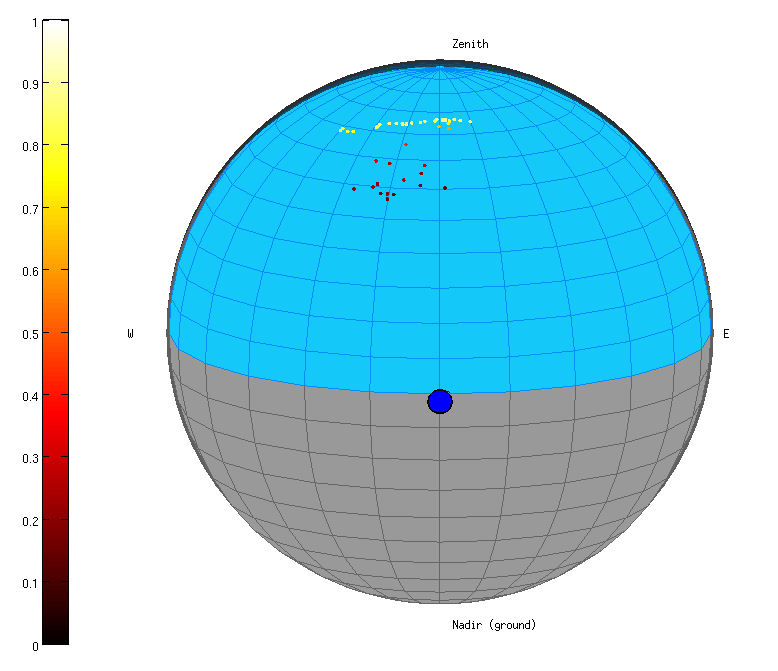
\includegraphics[width=0.32\linewidth]{selection_scaling/example_MLV.png} &
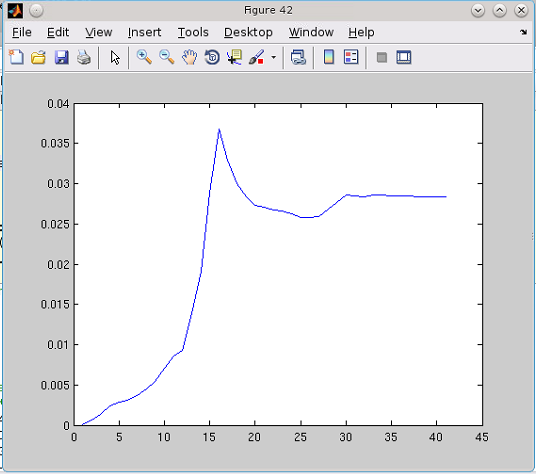
\includegraphics[width=0.32\linewidth]{selection_scaling/unordered.png} &
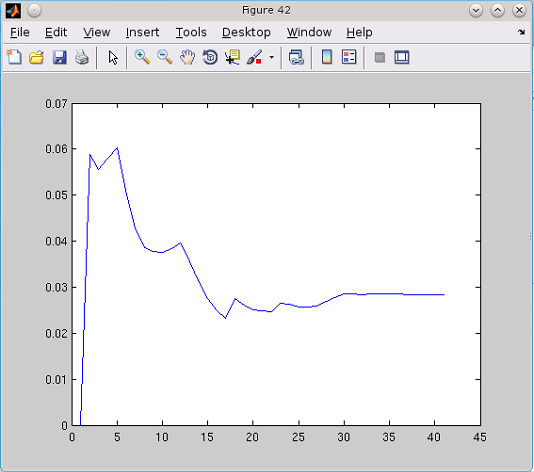
\includegraphics[width=0.32\linewidth]{selection_scaling/ordered.png} \\
(a) & (b) & (c)
\end{tabular}
\caption{\textbf{(a)} Evolution of Mean Light Vectors (MLV) over a day. \textbf{(b)} Condition number of the $\bar{L}$ matrix when taking the images ordered by time. The $x$-axis represents the number of images taken. \textbf{(c)} Same, but with images ordered by their importance, i.e., how their MLV span the space. Note how taking the whole sequence gives the same condition number, but the sequence in which they are presented can increase the condition number up to twice the maximum value obtained when ordered by acquisition time. \todo{Remake figures}}
\label{fig:sel-ordering}
\end{figure}

Even though this analysis shows promising results, it is based on the condition number and not a direct reconstruction performance assessment measure such as the uncertainty, as we used in our previous contributions. But even basing this analysis on the uncertainty won't give the best solution. This analysis is static, meaning that it orders the input images regardless of the quantity we aim for. Maybe a completely different subset of images than the sorted one would be optimal for a certain quantity of input image.

To solve this problem, I propose to transfer some knowledge from the linear algebra and machine learning domains to PS. From the linear algebra domain, Golub \emph{et al.}~\cite{Golub1977} studied the rank degeneracy of matrices in the least squares problem. From the machine learning domain, a whole area of research called ``feature selection'' is based on a similar idea. Both of them have a similar goal: to select some columns of a matrix while optimizing some property, such as the condition number. In order to do so, the common way to perform this is by matrix factorization. I plan on reviewing these two fields of studies to gain a global understanding of the problem. This will allow me to use the uncertainty as measure instead of the condition number, and to modify an existing algorithm to solve this problem.

Furthermore, once the optimal input images are selected, the conditioning of the problem may still be suboptimal. In that case, is there some processing that could be done on the images that could enhance the results? The bad conditioning can come from great variances in the lighting intensity. A common example is when the sun is shining at noon and a cloud occludes the sun in the afternoon. They both define a probably different MLV for a given normal. The second MLV can potentially be a very interesting vector spanning a section of the space yet unseen, but the intensity of the first one drowns it. This means that the first vector will have an norm significantly higher than the second vector. When taken in the least squares sense, the first vector will have more importance when solving than the second vector. But in reality, we don't what this to happen; both are valid pixel intensities gathered from the surface, explaining the first vector should be as important as explaining the second one.

This vector importance issue can be fixed by scaling the data by an arbitrary factor. By scaling both the input images and the computed MLVs to be of the same magnitude, the input images should be treated equally. Keeping in mind the impact of sensor noise, it is better to scale down the bright images than scaling up the dark images. The latter would boost the sensor noise, giving inaccurate data, and thus a high reconstruction uncertainty.


%\subsection{Shadow detection}
%3DV15 article with cool SD


\subsection{Algorithmic improvements}

% MRF, reference Jung's, tell our differences.
When performing a calibrated PS algorithm on environment maps, a chicken-and-egg problem arise. The part of the environment map visible by a surface patch is defined by its normal, but the normal is what we want to find using the lighting information. To solve this problem, as explained in our previous contributions, we can sample normals uniformly over the sphere and compute their MLVs. Then, we can fit how well a pixel intensity in the image matches these MLVs.

This scheme may work pretty well, but lacks a fundamental element: spatial coherence, which is very present in real world structures. As a way to enforce this, I propose to insert a new step to initialize the normals. To coarsely initialize the surface normals, the problem can be formalized as a Markov Random Field (MRF) by doing the hypothesis that a vertex normal is in some way related to its neighbors. This requires the definition of a unary and a pairwise term.

First, the unary term defines the cost of affecting a normal to a pixel. This unary term represents how well a normal explains the pixel intensity throughout the sequence of environment maps. This is done by computing the PS equation with the candidate normal and to compute its residual error. The residual error is the sum of all errors when predicting the pixel intensity from the MLVs over the image sequence. The higher this residual error is, the less the candidate normal explains well the pixel.

Then, the pairwise term defines the cost of a normal given its neighbors. A simple smoothness factor could be used, for example based on the angle between two evaluated normals. An interesting remark is made by~\cite{jung-cvpr-15}. Instead of the usual smoothness prior, one could base this pairwise terms on the likeness between pixels. They argue that pixels behaving similarly through the image sequence should also have similar surface normals. Technically, they base their similarity measure on the Pearson correlation coefficient. This promising idea is worth investigating.

The idea of using an MRF is to try all the sampled normals of the sphere on all the pixels. This will give one residual error per candidate normal. All these residual errors compose the unary term of the MRF. The chosen pairwise weights explained earlier link neighboring pixels. This gives a MRF formulation that can be optimized using a standard optimization technique~\cite{Boykov2001a,Kolmogorov2004a,Boykov2004,Bagon2006}.

While this MRF formulation was used recently to perform PS reconstruction~\cite{jung-cvpr-15}, it has been used only used as a final smoothing step to fix zones in shadow during most of the sequence. I believe this technique can be employed to initialize the PS procedure, followed by the standard fine-grained normal optimization, standard to PS algorithms.


% To do that, we'll need to merge some ideas from other techniques because sometimes, some pixels cannot be recovered. Silhouettes, Data-Driven priors.
The ideas previously conveyed will improve the reconstruction performance of outdoors PS and bring a better understanding of the impact of natural illumination on reconstruction algorithms based on photometric cues. But even if we improve a PS algorithm by a large margin, the analysis in our previous contributions showed that sometimes, even with the best possible surface with the lowest sensor noise, there is not enough photometric cues to recover certain normals or surfaces over the sphere.

To fix this issue, merging another technique with PS is the only choice. When data was captured on an unsuitable day, it will then be possible to still perform a 3D reconstruction. Previous work have shown that merging PS with Multi-View Stereo (MVS)~\cite{Beljan2012,Zhou2013,ackermann-3dv-14,HernandezEsteban2008,inose-tcva-13,shi-3dv-14} and even Structure from Motion (SfM)~\cite{zhang-iccv-03,lim-iccv-05} yield promising results. The difference between both technique is the calibration between the cameras. In Multi-View Stereo, the calibration of the cameras is known and the extrinsics between them is also known, while in Structure from Motion, the cameras are uncalibrated, which gives a projective ambiguity called the bas-relief ambiguity.

The idea I propose in the cases of unsolvable reconstruction using pure PS is to take some photos from another point of view, then performing a standard SfM algorithm to first get a coarse estimate of the scene. This will allow to fill the gaps with the dense result of PS that can constrain well on at least an axis in the worst case. For the other axis, the normal found by SfM can be propagated on neighboring vertices in conjunction with some smoothing regularization to obtain a final result.

The improvements described in this section are all planned to be part of a single PS algorithm. This algorithm will be the next contribution I plan to realize. While it won't be particularly practical on the field, as it needs the capture of the full environment map that lit the object to be reconstructed, it will bring enough improvements and novelty to lay the path for an uncalibrated version of it.

\section{Uncalibrated outdoor reconstruction}
\label{sec:uncalib}

% reconstruction, don't need lighting condition is a plus
All the proposed work up until now supposes we know the full environment map that lit the scene we observe. After the development of the fully calibrated algorithm described, I plan to overcome the need for capturing the sky. Getting rid of the lighting capture is a big plus, allowing the technique to be easily brought on the field. A single camera would be required, simplifying the capture apparatus by a great deal.

Uncalibrated PS reconstruction has an issue that its calibrated counterpart doesn't have: the Generalized Bas-Relief (GBR) ambiguity. Because the light intensity and direction as well as the surface albedo is not known beforehand, the reconstruction of the surface height is up to an unknown factor, impossible to determine without prior knowledge of the surface or constrains external to photometric cues.

%~\cite{basri-ijcv-2007}
Authors over the years have basically proposed two ideas to surmount the GBR ambiguity. Doing it manually (i.e., forcing a depth to an arbitrary value) seems to be a quite common way to deal with this issue. Most researchers, though, proposed a wide amount of priors and optimization schemes on the object material~\cite{tan-cvpr-07,alldrin-cvpr-08,abrams-eccv-12,queau-jmiv-14} to solve this problem.

% Data-driven approach, what can the DB tell us on the image.
%Bas-Relief Amb.
In order to make PS work uncalibrated, I plan to use a data-driven approach. By taking advantage of the sky database we already have, we can lead an algorithm to learn what a physically plausible sky looks like, constraining greatly the problem. The quantity of real world skies that can explain well enough the illumination on a scene is quite small, if we take the similar skies as one.

I suspect this lighting constraint to be enough to alleviate the GBR ambiguity issue. In the case this constraint is not enough, I plan to use an optimization method on the material albedo as proposed by the authors previously mentioned.

Overall, the GBR ambiguity is a minor issue with many techniques to solve it available in the literature. What is left to do, though, is an uncalibrated outdoor single day PS algorithm that brings performances similar to the laboratory conditions. The current state-of-the-art technique~\cite{jung-cvpr-15} obtains between 30\% and 40\% of the recovered normals under 30\degree of error, which is far away from the impressive precision obtained using PS in laboratory conditions.

In the following, I propose a succession of steps in order to take the calibrated algorithm proposed earlier and push it to a fully uncalibrated one.


\subsection{Half-calibrated case}
% First, reconstruction of the ground only.
A full environment map is hard to obtain. This means that a full sphere of irradiance must be captured. Usually, sky capture apparatus is composed of a wide angle lens pointing toward up (zenith), capturing only at best a small portion of the horizon. Building a full environment map is done by adding the ground, which requires the stitching of two captures.

The first enhancement to the system I propose is to get rid of the ground by estimating it. As of now, in our previous contributions we estimate the ground to be a single constant, repeated over the bottom (nadir) hemisphere. This is a good enough approximation on objects that have been laid carefully on a uniform piece of cloth, but is likely to break on real building-scale structures.

One thing that can be done is an 


\subsection{Mostly uncalibrated}
% Then, estimation of the sky using the GPS coordinates and date & time. Then, without date and time.
In order to move toward an uncalibrated algorithm, it feels a logical next step to remove the environment map altogether from the inputs of the method. To simplify a bit this big step, I propose to work with the GPS coordinates alongside with the date and time of image acquisition. This type of information is sometimes available (and sometimes right) in the EXIF data of pictures, making this kind of input not as farfetched as it may seem.

With the GPS coordinates and the date and time, it is possible to know where the sun should have been in the sky. With this information, it is possible to determine whether the sun is occluded by clouds or not, depending on the intensity of the object image. If it is not occluded, the MLV of pixels not in shadow are constrained to be on a circle at a fixed elevation. This circle is due to the unknown object rotation. While we can know with precision the position of the sun, the orientation of the camera is not known. One thing can be deduced, though: the elevation of this circle is the sun's elevation.

By using previous work on finding the low frequency illumination~\cite{basri-ijcv-2007} or by using matrix factorization techniques~\cite{shi-cvpr-10}, it is possible to know the maximum light direction. If we have at least one image where the sun is shining onto the object, is it then possible to assign this maximum light direction to the sun, resolving the rotation ambiguity.

The sky could then be estimated by a two component parametric model of the sky, like~\cite{jung-cvpr-15} did. But I propose instead to take advantage of our sky database in order to either find or synthesize a new sky explaining the observed scene. This approach has the advantage of producing real-looking physically-based environment maps.

Synthesizing new skies can be a complex task. When talking about synthesizing, the meaning is basically to find an environment map that fits globally the required specifications and, at need, rotate it so the energy comes from the desired directions. More advanced synthesizing techniques could be interesting to work with, for example generating a new environment map using texture synthesis, and will be tested if the need arise.

As an intermediate step, it is possible to remove the time as an input of the algorithm. Previously, we knew exactly the azimuth and elevation of the sun in the sky. Now, these values are constrained to an arc in the sky. I still assume the camera and object orientation are unknown. Now, using two images where the sun is not occluded, it is possible to solve this problem. Still using the maximum light direction technique, once two light directions are found, it is possible to find the camera azimuth (or object rotation). Using more images than two will provide an overconstrained system of equation, solvable using a standard least squares approach. As a bonus, the capture time can also be estimated.


\subsection{Fully uncalibrated}
% Lastly fully uncalibrated
The last step is to provide a fully uncalibrated PS algorithm. Building on the previously proposed technique, it is possible to remove the GPS coordinates and the date from the technique. It is expected that at least some captures over the sequence will be sunlit, yielding a high overall image intensity and giving a clear principal light direction using the maximum light direction scheme explained earlier. It is thus possible to find the sun arc in the sky, enabling self-calibration. By fitting these principal light directions to environment maps available in the database, it will be possible not only to obtain the scene structure but to estimate the lighting that made the photo.

This proposed technique will be a major contribution that iterates over the previous state of the art by adding a richer data-driven sky illumination model at its core.


\section{Looking farther than the sun}

% Up until now, we only considered the atmosphere during the day for reconstruction. The main problem, coplanar.
All the previous proposed work only considered the atmosphere during the day. The main problem, which is the coplanarity of the sun trajectory over the course of a day, can be solved by richer and more complex sky models as explained in the previous sections. Another interesting avenue is to revert to a simpler model: the point light source. In this case, using solely the sun as a light source will, most of the time, give an underconstrained problem that will not perform well.

With this analysis, though, it is necessary to bring something else into play in order to better constrain the problem. It is hard to find something capable of competing with the sun in terms intensity in the sky through a day, but the moon can be up to par in terms of quantity of information needed to constrain the problem correctly.
%Another avenue is to manually modify the lighting, either by distorting the sun light or adding new light sources.


\subsection{Day \& Night PS}
When seen during the day, the moon doesn't bring much lighting to a scene. But during the night, it can be strong enough to cast clearly visible and sharp shadows on the ground. But the main interesting thing about the moon is that it presents lighting from a plane different than the sun. Using this to our advantage could turn a data capture failure for PS (e.g., during a fully sunny day) into a successful reconstruction, by simplifying the illumination model and letting the capture continue overnight.

Over the course of 24 hours, both sun and moon trajectories are mostly coplanar. Examples of such trajectories are shown in fig.~\ref{fig:DN-sunmoon-trajectories}. Both of them are parallel, which is not surprising because the earth, the sun and the moon are roughly on the same plane in the solar system. But the inclination of the earth makes both trajectories superposed in the sky during the equinoxes, which occurs around 81 days (spring) and 264 days (fall) after January 1st.

\begin{figure}
\centering
\begin{tabular}{cc}
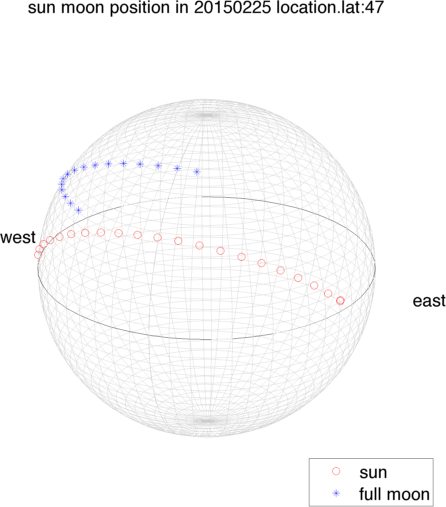
\includegraphics[height=0.49\linewidth]{DayNight/20150225_lat47.png} &
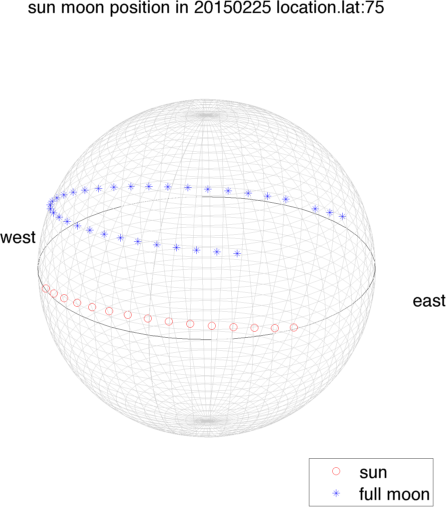
\includegraphics[height=0.49\linewidth]{DayNight/20150225_lat75.png} \\
a) & b)
\end{tabular}
\caption{Example of the trajectories of the sun and the moon for 2015-02-25 at latitude a) 47 and b) 75. Two things are interesting to note: First, the moon trajectory suddenly stops because the sun rises at this moment. The moon is then not considered as a dominant light source anymore. Secondly, as the latitude gets higher, the trajectories becomes more and more parallel to the horizon.}
\label{fig:DN-sunmoon-trajectories}
\end{figure}

The measure used to analyze the PS reconstruction quality using both the sun and the moon is called the maximum gain. This maximum gain is the factor that multiplies the sensor noise, as explained in the previous contributions. The higher it is, the more uncertain (or wrong) the reconstruction will be. So the lower is the maximum gain, the better will be the reconstruction performance.

%and fig.~\ref{fig:DN-maximum_gain_latitude} \todo{for most of earth latitudes}
Such an analysis for year 2015 is found in fig.~\ref{fig:DN-maximum_gain} for the location of University Laval. As we can see, the two major peaks around days 81 and 264 are explained by the equinox trajectory alignment. Since both trajectories are almost superposed, the system of equations is pretty badly conditioned, leaving a high maximum gain. Another interesting thing to notice is the small sinusoid with a 29.54 days period present over the whole year. This happens when not much of the moon is visible during a night, for example when rising at 4 am during a summer night. Since the sun's dawn is pretty near, the moonlit duration is small, giving only a small arc of the moon plane. When this happens, the maximum gain increases because both arcs are not fully seen. The increase is not so bad when far from the equinoxes, because at least one capture is available with the moon as major light source. This reduces the problem to a matrix of coplanar vectors -- caused by the sun -- augmented by (at least) a single vector outside of this plane -- caused by the moon --, which is enough to constrain the problem.

\begin{figure}
\centering
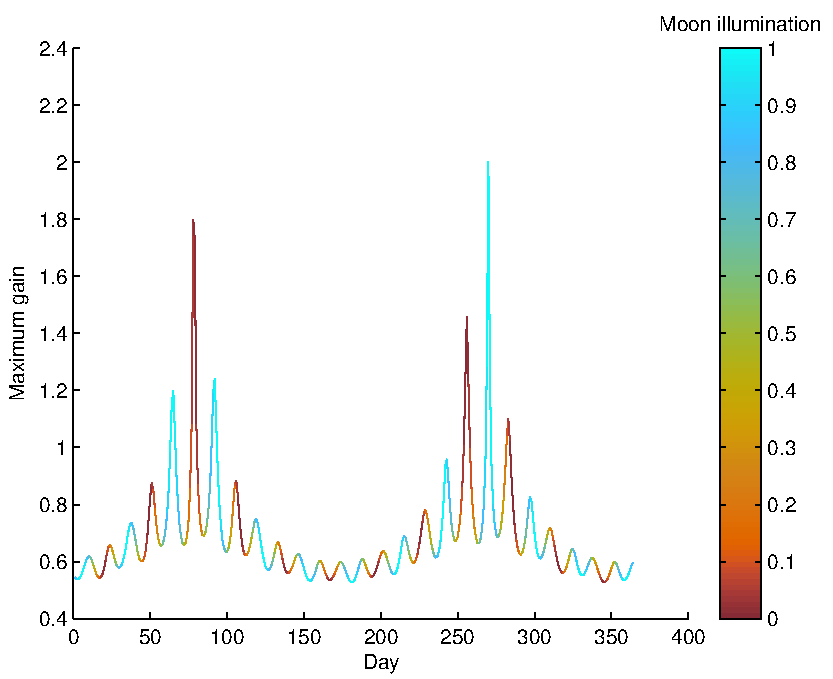
\includegraphics[height=8cm]{DayNight/maximum_gain.pdf}
\caption{Maximum gain for PS reconstruction assuming an illumination of 24 hours (sun and moon) for the year 2015. The color-coded moon illumination represent the phase of the moon, full moon being 1 and new moon being 0. The location is the University Laval Campus (Latitude and Longitude = 46.779077, -71.275778 ). }
\label{fig:DN-maximum_gain}
\end{figure}

%\begin{figure}
%\centering
%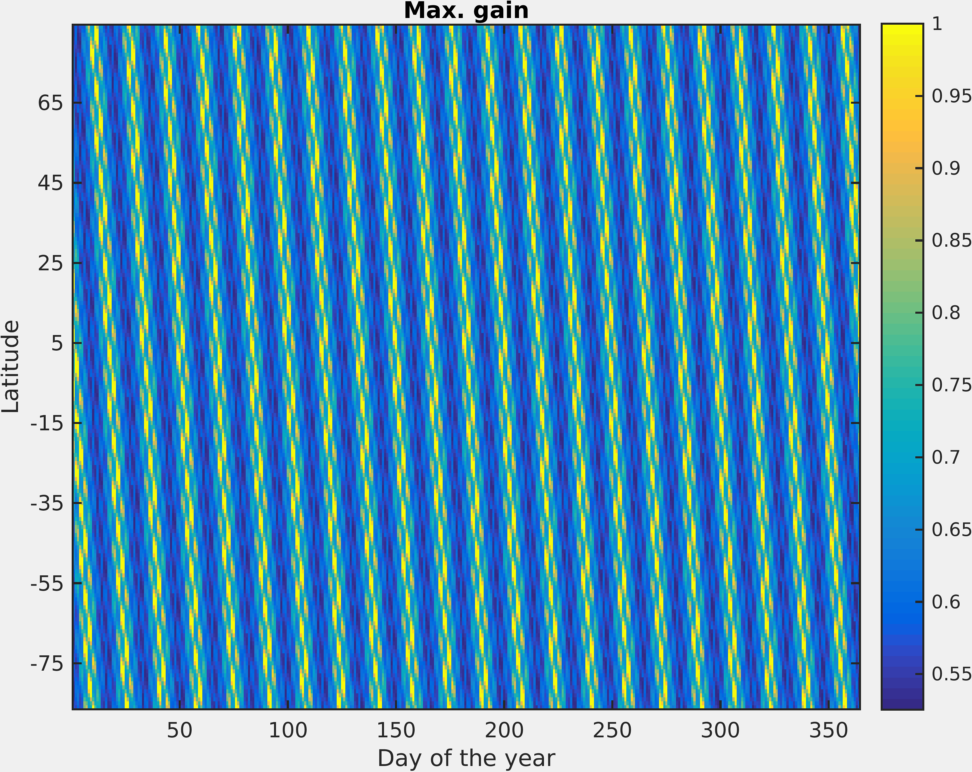
\includegraphics[height=8cm]{DayNight/maximum_gain_over_latitude.png}
%\caption{Maximum gain in function of the day for the year 2015 and the latitude of the observer. This gain is clipped to 1.}
%\label{fig:DN-maximum_gain_latitude}
%\end{figure}

Another notion worth of mention is the moon illumination. Over the course of its cycle, the moon will have an illumination of
\begin{equation}
k = \frac{1 + \cos(\phi)}{2}  \quad,
\end{equation}
where $\phi$ is the lunar phase in radians~\cite{Meeus1991}. While this idea will obviously not work when the illumination is null, the rest of the time, the reconstruction performance will be highly dependent upon the light pollution at the capture location. This light pollution can be approximated by an ambient illumination term, which is analyzed by~\cite{Angelopoulou2013}.

Statues, historical bridges and architectural monuments are often lit using spotlights during the night. During a new moon, such spotlights could be used as substitutes to the moon in this analysis, providing another way to constrain correctly the PS problem.

The main problem with this idea, as can be seen from the unusual astronomical arguments made in this section, is the knowledge transfer between the astronomical domain and computer vision. We can assume that most of the people aware of PS have little to no knowledge of the side effects of the cycle of the moon and its trajectory in the sky. By investigating this field of study and summarizing the pertinent informations, I am certain that performing day \& night PS will bring a nice contribution to the community. Furthermore, knowledge gained in low lighting conditions such as the night will likely be profitable on some daylight illumination, such as cloudy days.


%\subsection{Artificial alterations}

%The sun, when taken as a point light source, may have a coplanar trajectory over the course of a day, but nothing prevents the addition or modification of this lighting.

% Diffusers

% City lights


%\subsection{Other techniques}



%\section{Augmentation avec d'autres techniques}

% from ICCP
%While these techniques can lead to well-defined solutions, they are not always practical in many scenarios with strict temporal or geographical constraints. A second strategy has therefore been to combine PS with other techniques such as multi-view stereo~\cite{inose-tcva-13,shi-3dv-14}, or use reference objects as in \cite{johnson-cvpr-11} or example-based PS~\cite{hertzmann-pami-05,ackermann-3dv-14}. But can we accurately reconstruct surface geometry simply based on the photometric cue in an outdoor setting, without overly restrictive temporal and geographical constraints?

%Décrire l'amélioration que pourrait apporter la PS utilisée conjointement avec du SFM et la stéréo multivues standard.